\documentclass[dp]{FEIstyle}
\usepackage[textsize=tiny]{todonotes}

\usepackage{tocbibind}
\usepackage{booktabs}
\usepackage{lscape}

%\usepackage{encxvlna} % predlozky na konci riadku
\usepackage{luavlna}
\usepackage{setspace}
\usepackage{tabularx}
% upravene premenne oproti defaultu

\FEIschool{Paneurópska vysoká škola}
\FEIfaculty{Fakulta informatiky}

%

\FEIauthor{Bc. Peter Drábik}
\FEItitle{Využitie MS HOLOLENS 2 vo vzdelávaní}
% \FEItitleEn{Example \LaTeX\ document with long title}
\FEIkeywords{Microsoft HoloLens 2, zmiešaná realita, nervová sústava, Unreal Engine, biológia, vyučovanie}
\FEIkeywordsEn{Microsoft HoloLens 2, mixed reality, nervous system, Unreal Engine, biology, teaching}
\FEIregNr{FI-100786-21449}
\FEIsupervisor{RNDr. Ján Lacko, PhD.}
\FEItrainingWorkplace{Ústav aplikovanej informatiky}
\FEIdate{7}{1}{2024}
%\FEIconsultant{Ing. John Doe}

\FEIglossaries{includes/glossary}
\bibliography{includes/bibliography.bib}

%\glsenablehyper
\captionsetup[table]{
  justification=centering,
  singlelinecheck=false % To center even if the caption is a single line
}


\iffalse \newacronym{crt}{CRT}{Cathode-Ray Tube}
\newacronym{ar}{AR}{Augmented Reality}
\newacronym{vr}{VR}{Virtual Reality}
\newacronym{mr}{MR}{Mixed Reality}
\newacronym{lbs}{LBS}{Laser Beam Scanning}
\newacronym{mrtk}{MRTK}{Mixed Reality Toolkit}
\newacronym{ui}{UI}{User Interface}
\newacronym{ux}{UX}{User Experience}
\newacronym{foss}{FOSS}{Free and Open Source Software}
\newacronym{fps}{FPS}{First-Person Shooter}
 \fi

\begin{document}

\pagestyle{empty} %%%%%

\frontmatter

\FEIpdfInfo
\FEIcover
\FEItitlePage
%\FEIassignment{includes/zadanie.png}
\FEIassignmentCustom
\newpage
% \FEIassignment{includes/assignment_part2.jpeg}
\FEIthanks{includes/thanks}
\FEIprehlasenie{}
\FEIabstract{includes/abstract}
\FEIabstractEn{includes/abstractEN}


\FEIcontent
%\FEIlistOfFiguresAndTables
\renewcommand{\listfigurename}{Zoznam ilustrácií} 
\renewcommand{\cftloftitlefont}{\bf\fontsize{22pt}{20pt}\selectfont} % kopia zo \sectionfont
\renewcommand{\cftfigpresnum}{Obr\'{a}zok\ }

\newlength{\mylenf}
\settowidth{\mylenf}{\cftfigpresnum}
\setlength{\cftfignumwidth}{\dimexpr\mylenf+3em}
\setlength{\cfttabnumwidth}{\dimexpr\mylenf+3em}

\FEIlistOfFigures
\FEIlistOfGlossaries
%\FEIlistOfAlgorithms
%\FEIlistOfListings

\mainmatter

\pagestyle{plain}  %%%%%%

\FEIintroduction{includes/introduction}
\FEIcore{includes/core}
\FEIconclusion{includes/conclusion}
% \FEIresume{includes/resume} % Use only iff document is in english language

% bibliography should use UTF-8 accents (write as is ľščťžýáí...) NOT converted by BibDesk
% http://tex.stackexchange.com/questions/57743/how-to-write-%C3%A4-and-other-umlauts-and-accented-letters-in-bibliography
\FEIbibliography %includes/bibliography.bib

\backmatter

%\FEIlistOfAppendix
%\FEIappendix{Štruktúra elektronického nosiča\label{att:A}}{includes/attachmentA}
%\FEIappendix{Algoritmus\label{att:B}}{includes/attachmentB}
%\FEIappendix{Výpis sublime\label{att:C}}{includes/attachmentC}

%\FEIappendix{Niagara Module Script\label{att:nms}}{includes/attachment-1}

\noindent\cleardoublepage
\phantomsection 
\addcontentsline{toc}{section}{Prílohy}
\section*{Prílohy}
\begin{enumerate}[leftmargin=*]
    \item Niagara Module Script \label{att:nms}
    \begin{figure}[!htbp]
        \centering
        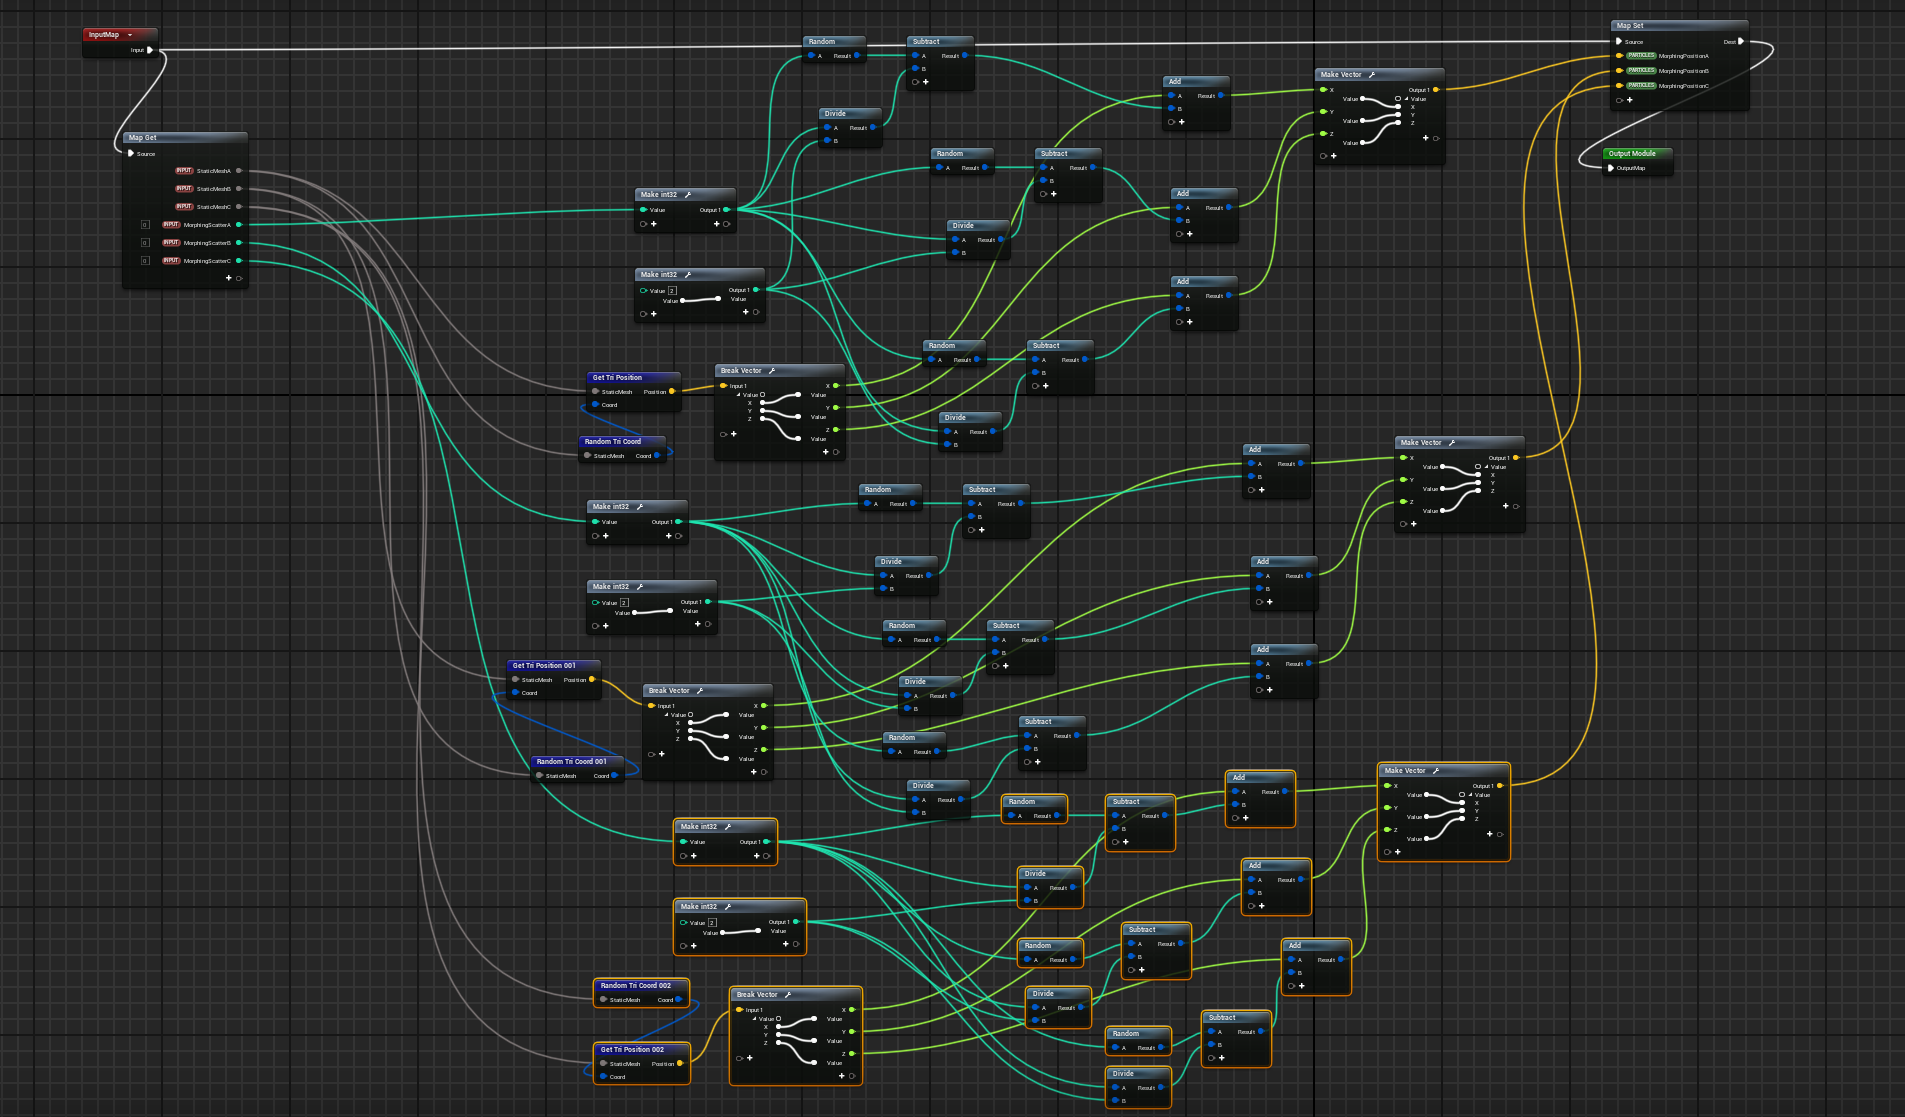
\includegraphics[width=21cm,angle=90,origin=c]{img/nms.png}
    \end{figure}
    \newpage

    \item Blueprint \texttt{Niagara\_3Lerp} \label{att:lerp}
    \begin{figure}[!htbp]
        \centering
        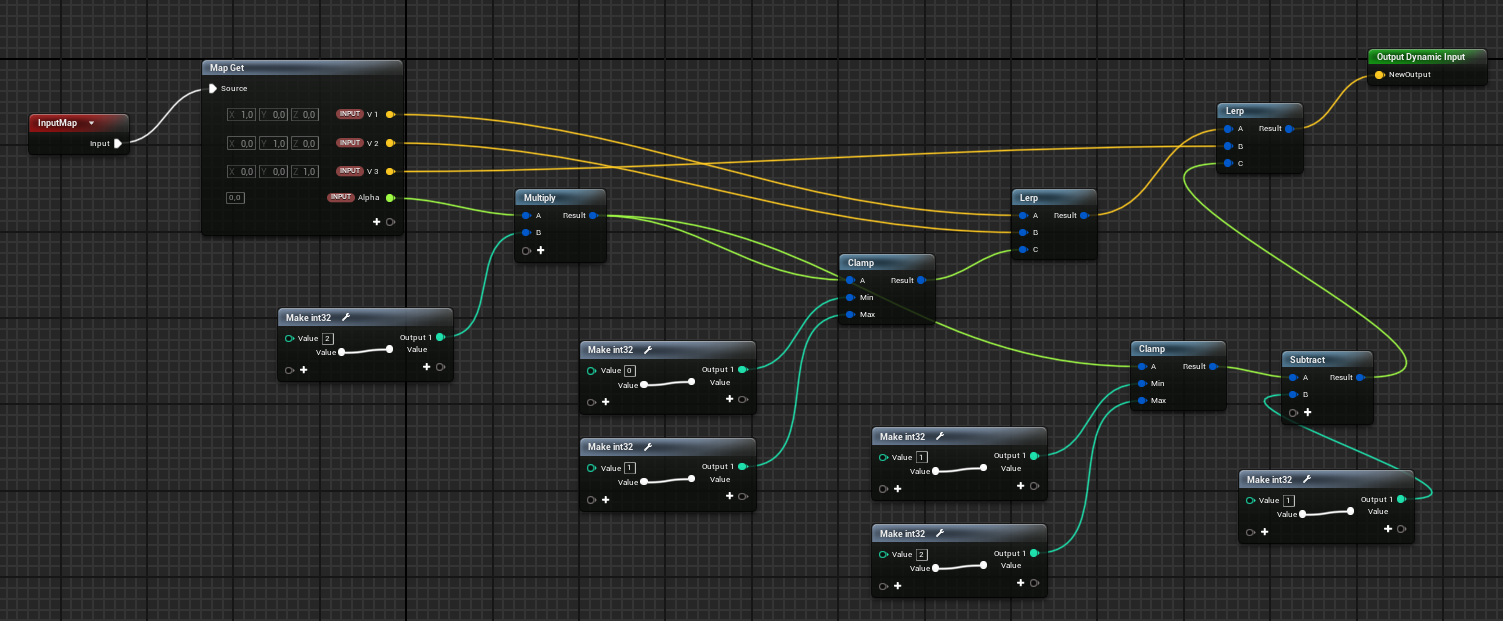
\includegraphics[width=22cm,angle=90,origin=c]{img/3lerp.png}
    \end{figure}
    \newpage

    \item Skript s časovou osou v Blueprinte \texttt{BP\_Neuron} \label{att:main-animate}
    \begin{figure}[!htbp]
        \centering
        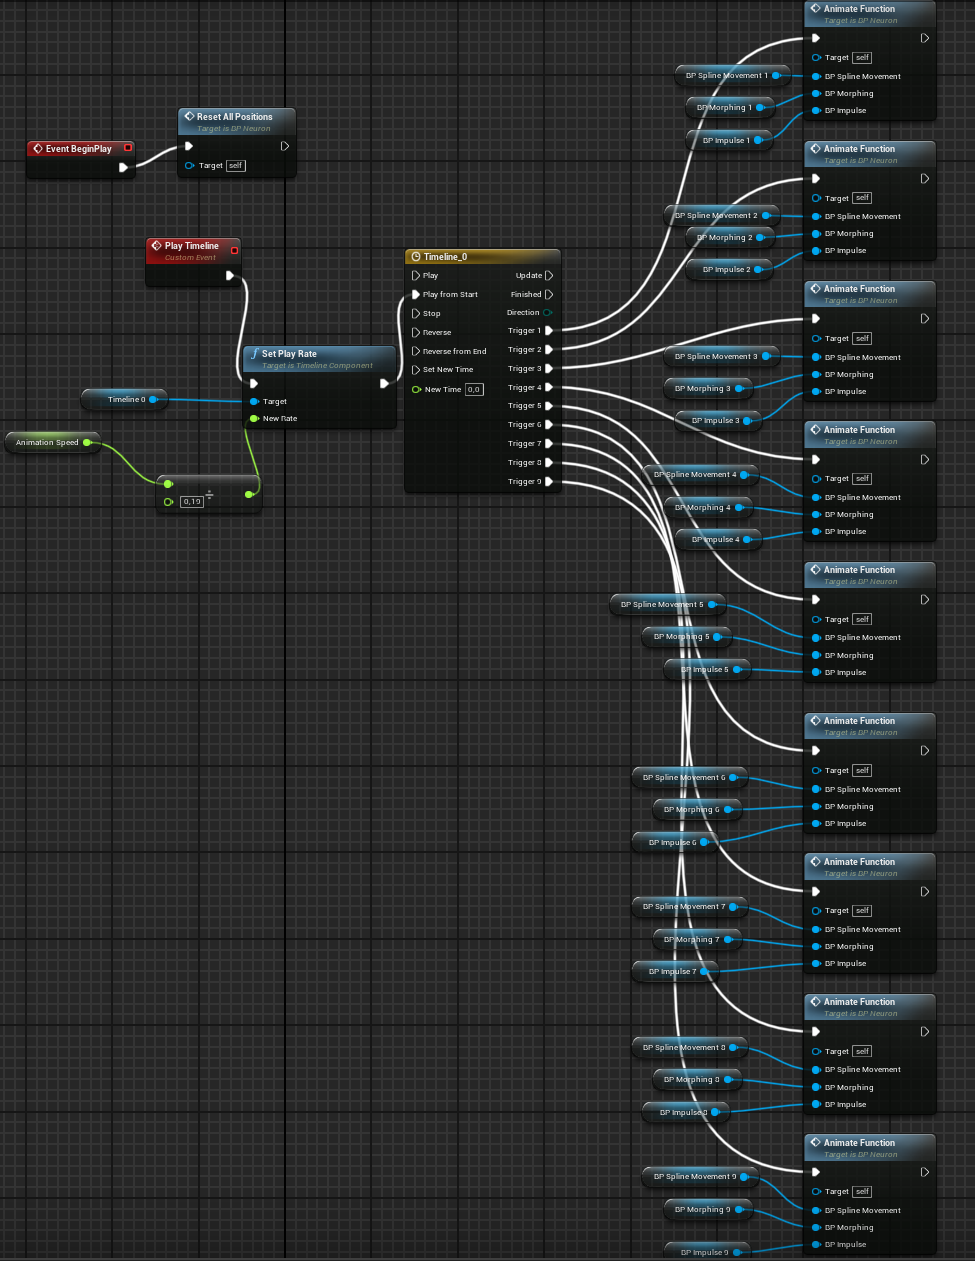
\includegraphics[width=16cm]{img/main-animate.png}
    \end{figure}
    \newpage

    \item Dotazník {--} položky 1 a 2 \label{att:dot1}
    \begin{figure}[!htbp]
        \centering
        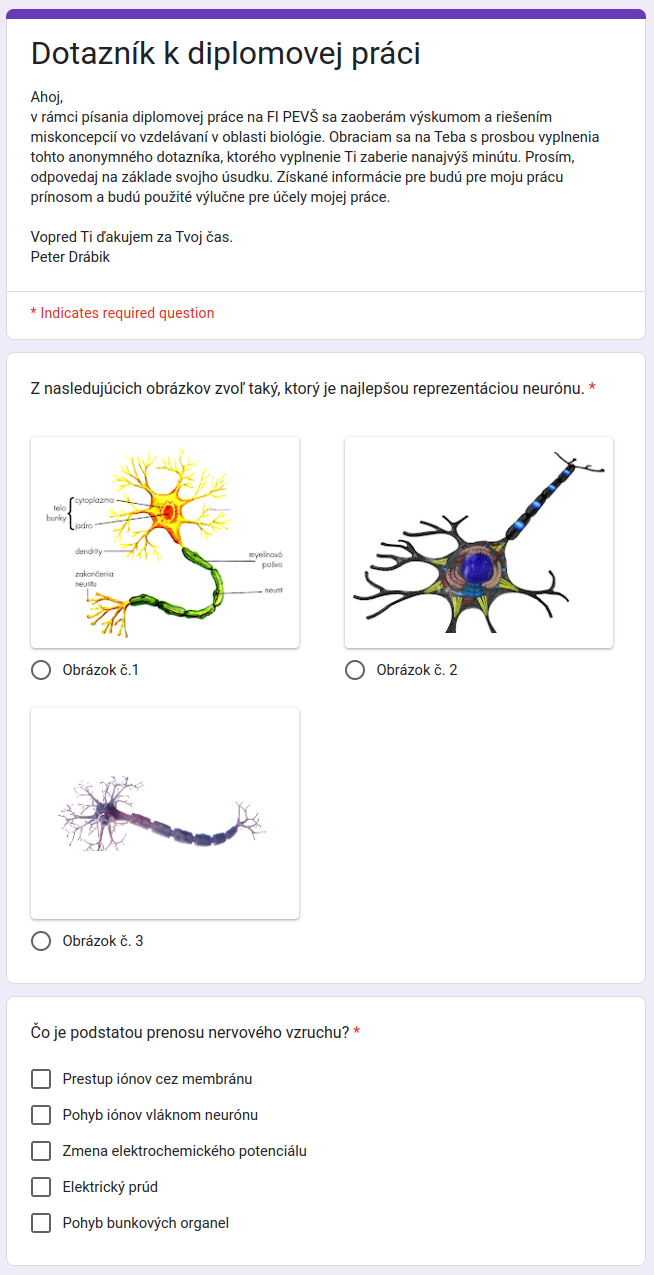
\includegraphics[width=11cm]{img/dot1.png}
    \end{figure}
    \newpage

    \item Dotazník {--} položky 3, 4 a 5 \label{att:dot2}
    \begin{figure}[!htbp]
        \centering
        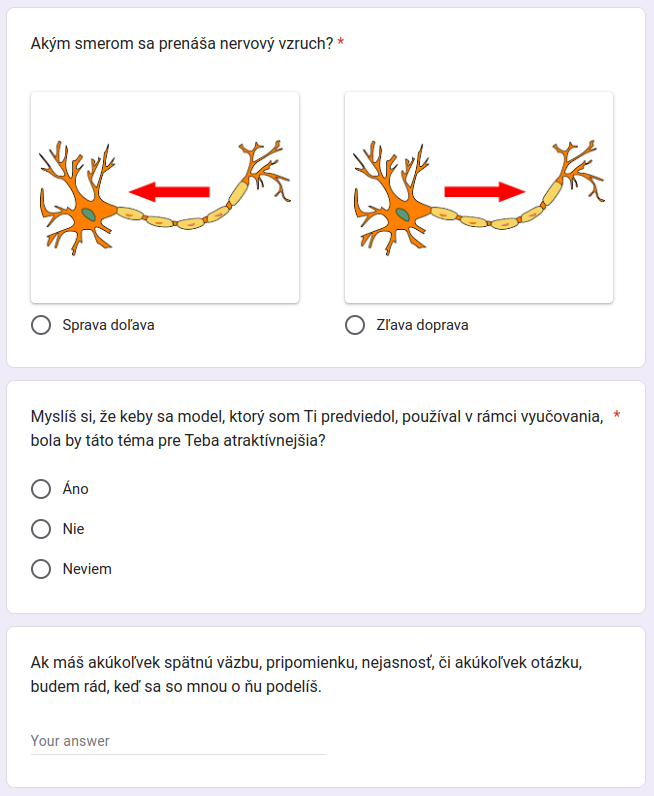
\includegraphics[width=14cm]{img/dot2.png}
    \end{figure}
    \newpage

\end{enumerate}

\end{document}